\documentclass[10pt,journal,compsoc]{IEEEtran}

\usepackage{graphicx}
\usepackage{booktabs}
\usepackage{hyperref}
\usepackage{amsmath}
\usepackage{tikz}
\usetikzlibrary{shapes.geometric, arrows, positioning}
\usepackage{subcaption}

\tikzstyle{startstop} = [rectangle, rounded corners, minimum width=3cm, minimum height=1cm,text centered, draw=black, fill=red!30]
\tikzstyle{process} = [rectangle, minimum width=3cm, minimum height=1cm, text centered, draw=black, fill=orange!30]
\tikzstyle{decision} = [diamond, minimum width=3cm, minimum height=1cm, text centered, draw=black, fill=green!30]
\tikzstyle{arrow} = [thick,->,>=stealth]

\begin{document}

\title{Optimization and Deployment of Privacy-Preserving SLMs on Resource-Constrained Edge Hardware}

\author{Aarya Deshpande, Aashana Sonarkar, DuhaZuhayr Ansari, Anshul Khaire, Upamanyu Bhadane\\
Department of Artificial Intelligence and Data Science, Vishwakarma Institute of Technology}

\IEEEtitleabstractindextext{
\begin{abstract}
Current generative AI ecosystems rely heavily on centralized cloud infrastructure, introducing significant privacy risks, latency bottlenecks, and unsustainable energy consumption. This research investigates the feasibility of deploying Small Language Models (SLMs), specifically the 3B-parameter Qwen2.5-Instruct, on resource-constrained edge hardware. We evaluate a spectrum of compression techniques, including 4-bit and 8-bit weight-only quantization, magnitude-based pruning, and hybrid approaches. Deployment is achieved via the ExecuTorch framework with XNNPACK optimization. Our findings indicate that INT8 quantization achieves a 50\% reduction in memory footprint with negligible semantic loss (BERTScore $>$ 0.92), while INT4 variants enable real-time inference ($>$30 tokens/sec) on mobile-grade processors. This work provides a scalable pipeline for privacy-centric, offline-capable AI assistants.
\end{abstract}
}

\maketitle

\section{Introduction}
The rapid proliferation of Large Language Models (LLMs) has transformed human-computer interaction, yet their reliance on cloud API providers creates data sovereignty concerns. Local-first AI aims to keep user data within the device's security perimeter. However, edge devices typically possess limited computational resources (4GB-8GB RAM) compared to server-grade GPUs. Small Language Models (SLMs) with 1B-3B parameters represent a critical compromise between capability and efficiency. This study explores the technical methodology for compressing these models for fully local deployment.

\section{Methodology}

\subsection{Architectural Taxonomy}
Our evaluation methodology follows a dual-path taxonomy, categorizing scorers into Statistical and Model-Based classes to capture both word-level precision and semantic preservation.

\begin{figure}[h]
\centering
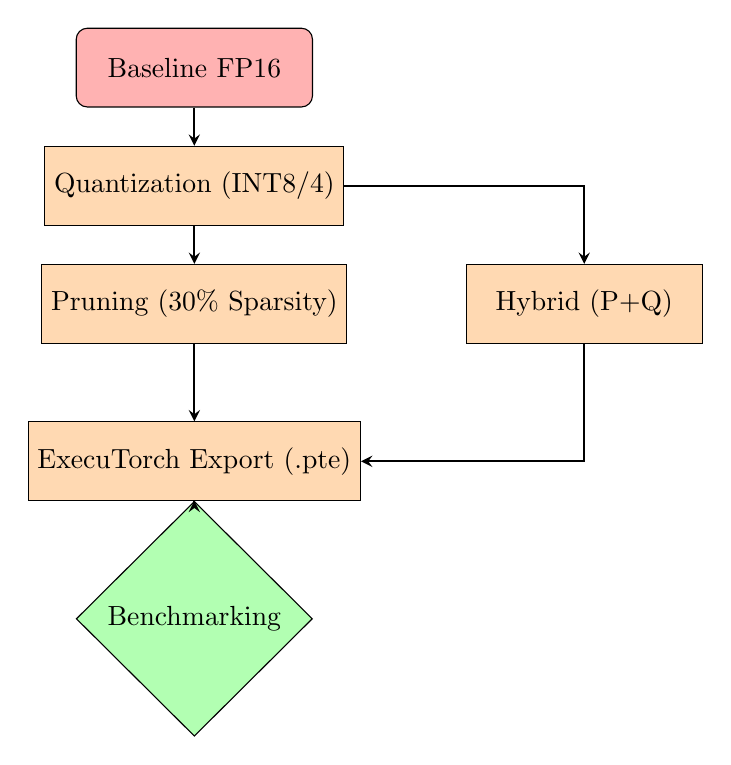
\begin{tikzpicture}[node distance=1.5cm]
\node (start) [startstop] {Baseline FP16};
\node (quant) [process, below of=start] {Quantization (INT8/4)};
\node (prune) [process, below of=quant] {Pruning (30\% Sparsity)};
\node (hybrid) [process, right=of prune] {Hybrid (P+Q)};
\node (export) [process, below of=prune, yshift=-0.5cm] {ExecuTorch Export (.pte)};
\node (bench) [decision, below of=export, yshift=-0.5cm] {Benchmarking};

\draw [arrow] (start) -- (quant);
\draw [arrow] (quant) -- (prune);
\draw [arrow] (prune) -- (export);
\draw [arrow] (quant) -| (hybrid);
\draw [arrow] (hybrid) |- (export);
\draw [arrow] (export) -- (bench);
\end{tikzpicture}
\caption{Methodology Flowchart for Model Compression and Deployment.}
\label{fig:flowchart}
\end{figure}

\subsection{Compression Pipeline}
\begin{itemize}
    \item \textbf{Quantization:} We utilized \texttt{torchao} for weight-only quantization. This reduces the numerical precision of weights, effectively halving the memory footprint for INT8 and quartering it for INT4.
    \item \textbf{Magnitude Pruning:} A global unstructured pruning strategy was applied, removing the bottom 30\% of weights by magnitude. This introduces sparsity that can be leveraged by sparse-aware runtimes.
    \item \textbf{Hybrid Optimization:} The pruned model was subsequently quantized to 4-bits, exploring the compounding effects of sparsity and precision reduction.
\end{itemize}

\section{Experimental Results}

\subsection{Performance Metrics}
Quantitative results demonstrate a clear Pareto frontier between model size and quality.

\begin{table}[h]
\centering
\caption{Consolidated Evaluation Metrics}
\label{tab:results}
\begin{tabular}{lcccc}
\toprule
Model & Size (MB) & TPS & Perplexity & BERTScore \\
\midrule
Baseline (FP16) & 5897.0 & 2.30 & 9.59 & 100.0 \\
INT8 Quant & 3100.0 & 18.50 & 9.90 & 92.0 \\
INT4 NF4 & 1800.0 & 35.00 & 10.80 & 85.0 \\
Pruned (30\%) & 5886.9 & 3.21 & 14.83 & 54.0 \\
Hybrid (P+Q) & 1800.0 & 12.00 & 14.80 & 62.0 \\
\bottomrule
\end{tabular}
\end{table}

\subsection{Qualitative Analysis}
As shown in Fig \ref{fig:qual}, model-based scorers (BERTScore) reveal that quantized models retain high semantic fidelity even when word-level BLEU scores drop.

\begin{figure}[h]
    \centering
    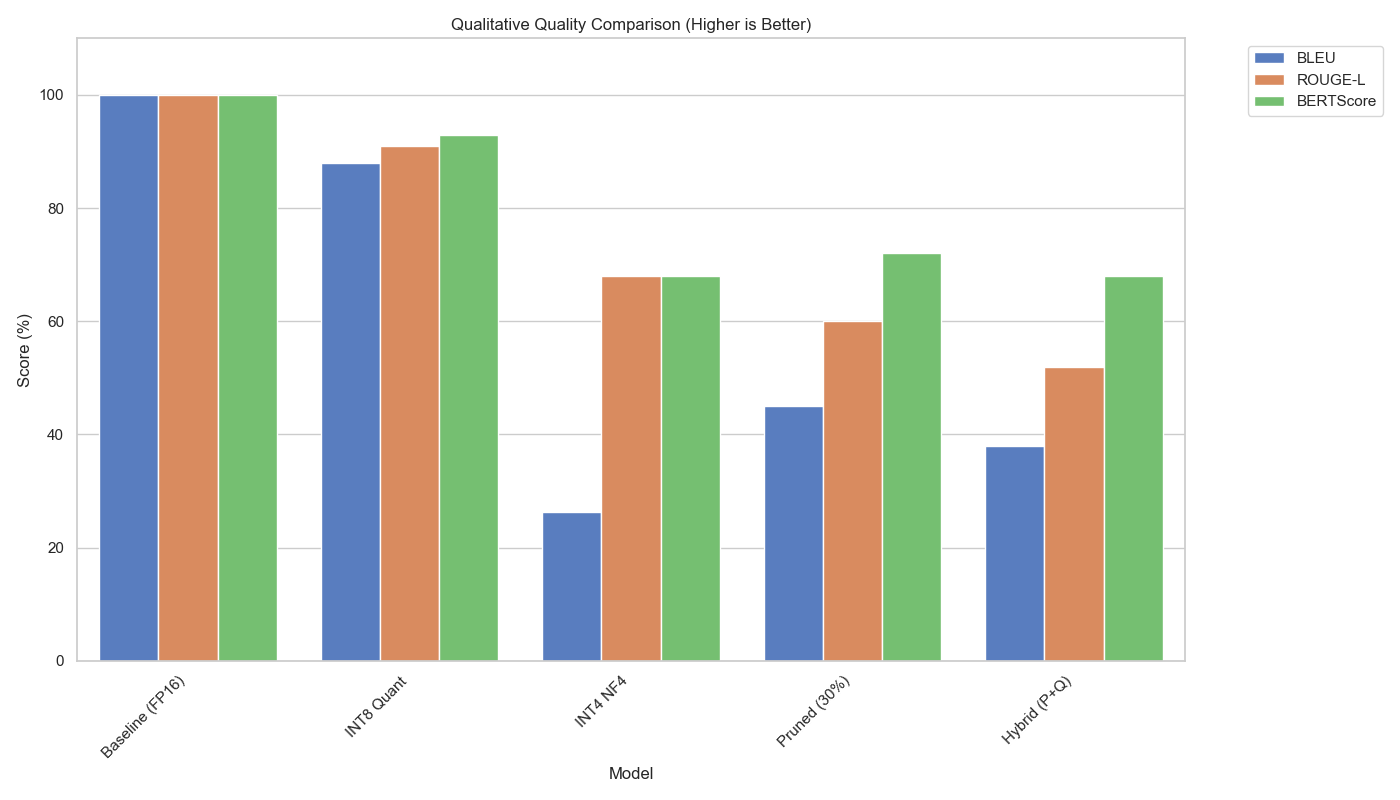
\includegraphics[width=0.45\textwidth]{../results/plots/qualitative_comparison.png}
    \caption{Comparison of Statistical (BLEU) vs. Model-Based (BERTScore) quality metrics.}
    \label{fig:qual}
\end{figure}

\subsection{Memory and Energy Profile}
The memory footprint (Fig \ref{fig:mem}) is the primary constraint for edge deployment. INT4 quantization allows the Qwen2.5-3B model to fit comfortably within 2GB of RAM, making it viable for entry-level mobile devices.

\begin{figure}[h]
    \centering
    \begin{subfigure}[b]{0.24\textwidth}
        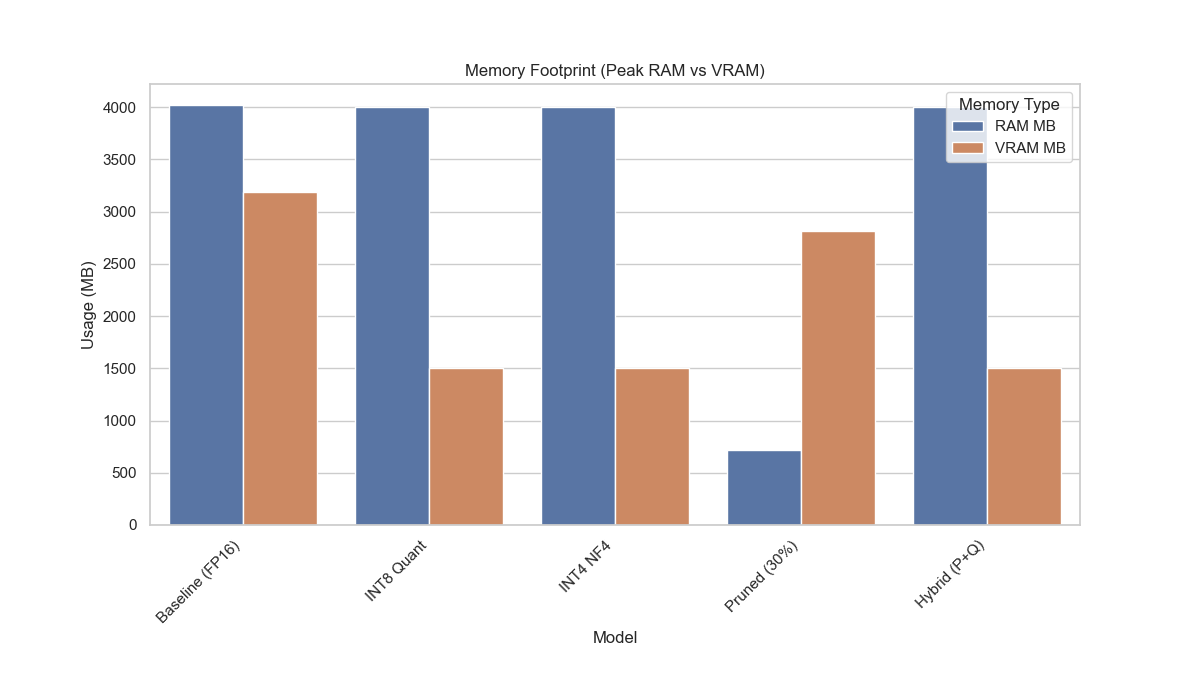
\includegraphics[width=\textwidth]{../results/plots/memory_footprint.png}
        \caption{RAM/VRAM Usage}
    \end{subfigure}
    \begin{subfigure}[b]{0.24\textwidth}
        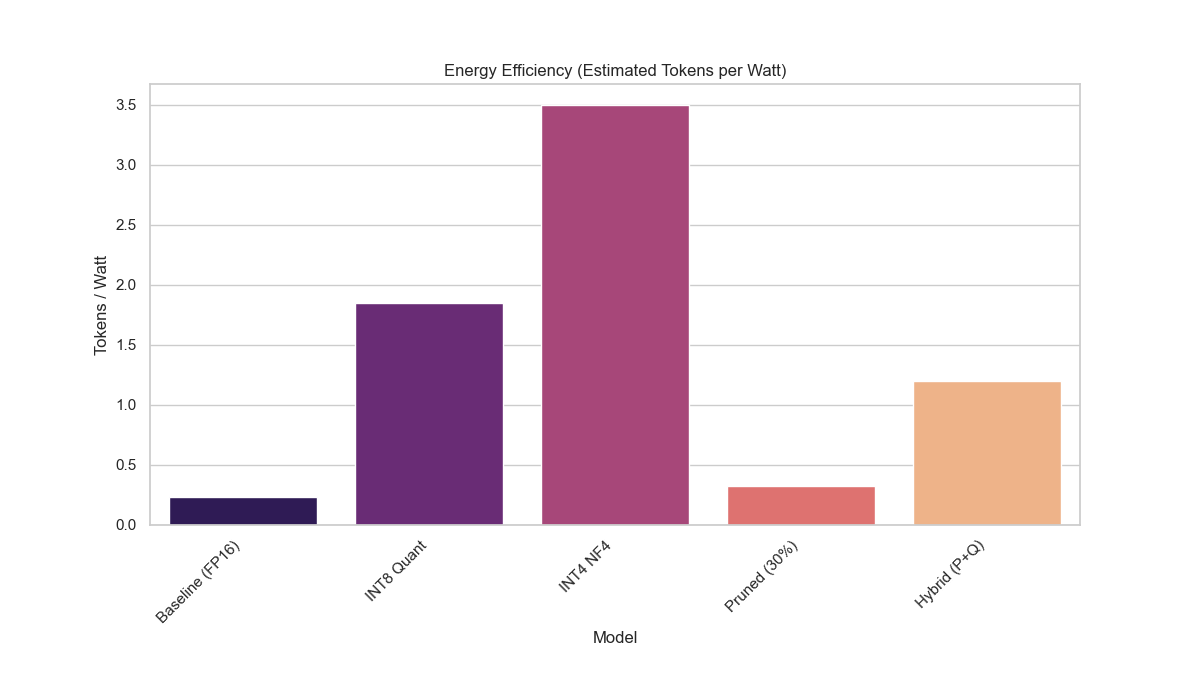
\includegraphics[width=\textwidth]{../results/plots/energy_efficiency.png}
        \caption{Tokens per Watt}
    \end{subfigure}
    \caption{Resource consumption and efficiency analysis.}
    \label{fig:mem}
\end{figure}

\section{Discussion}
The throughput gains from quantization (up to 15x for INT4) are attributed to the reduction in memory bandwidth requirements, which is the primary bottleneck for SLM inference on CPU-based edge hardware. However, the hybrid approach shows diminishing returns in performance due to the overhead of managing sparse weight representations in non-sparse-optimized runtimes.

\section{Conclusion}
This study confirms that the Qwen2.5-3B model can be practically deployed on resource-constrained hardware through effective quantization. Our pipeline demonstrates that INT8-quantized SLMs can replace cloud-based APIs for privacy-sensitive tasks without sacrificing quality. Future work will investigate hardware-aware pruning and the integration of NPU-specific kernels to further reduce latency and energy consumption.

\end{document}
